%\pdfoutput=1
% Uncomment line above if submitting to arXiv and using pdflatex

% $Id: main.tex 33041 2013-03-25 16:12:53Z tgershon $
% ============================================================================
% Purpose: Template for LHCb documents
% Authors: Tomasz Skwarnicki, Roger Forty, Ulrik Egede
% Created on: 2010-09-24
% ============================================================================
\documentclass[12pt, a4paper, twoside]{book}


% Variables that controls behaviour
\usepackage{ifthen} % for conditional statements
\newboolean{pdflatex}
\setboolean{pdflatex}{true} % False for eps figures

\newboolean{articletitles}
\setboolean{articletitles}{true} % False removes titles in references

\newboolean{uprightparticles}
\setboolean{uprightparticles}{false} %True for upright particle symbols

\newboolean{inbibliography}
\setboolean{inbibliography}{false} %True once you enter the bibliography

% THis file contains all the default packages and modifications for
% LHCb formatting

%% %%%%%%%%%%%%%%%%%%
%%  Page formatting
%% %%%%%%%%%%%%%%%%%%
\usepackage[inner=2.9cm,outer=2.6cm,bottom=2.6cm]{geometry}

\raggedbottom
% To avoid Latex to be too fussy with line breaking ...
\sloppy

%%% Header
\usepackage{fancyhdr}
\pagestyle{fancy}
\fancyhead[RO,LE]{}
\fancyhead[LO]{\itshape \nouppercase\leftmark}
\fancyhead[RE]{\itshape \nouppercase\rightmark}
\setlength{\headheight}{15pt}


%%At the beginning of chapter make half page free space
%\usepackage{setspace}
%\onehalfspacing

%% %%%%%%%%%%%%%%%%%%%%%%%
%% Packages to be used
%% %%%%%%%%%%%%%%%%%%%%%%%
\usepackage{microtype}
\usepackage{lineno}  % for line numbering during review
\usepackage{xspace} % To avoid problems with missing or double spaces after
\usepackage{ulem}
%\usepackage{hepnames}

%% Graphics
\usepackage{graphicx}  % to include figures (can also use other packages)
\usepackage{color}
\usepackage{xcolor}
\usepackage{colortbl}
\usepackage{rotating}
\usepackage{subfigure}
\usepackage{epstopdf}
\graphicspath{{./figs/}} % Make Latex search fig subdir for figures

%%Tables
\usepackage{longtable} % only for template; not usually to be used in PAPERs
\usepackage{multirow}


%% Math
\usepackage{amssymb,amsfonts,amsmath,mathtext}
\usepackage{amsmath} % Adds a large collection of math symbols
\usepackage{amssymb}
\usepackage{amsfonts}
\usepackage{upgreek} % Adds in support for greek letters in roman typeset
\usepackage{breqn} %%two lines in formulas

%%Diagamms
\usepackage{tikz}
\usetikzlibrary{decorations.pathreplacing,decorations.pathmorphing,decorations.markings,trees,calc,patterns,decorations}

%% fix to allow peaceful coexistence of line numbering and
%% mathematical objects
%% http://www.latex-community.org/forum/viewtopic.php?f=5&t=163
%%
\newcommand*\patchAmsMathEnvironmentForLineno[1]{%
\expandafter\let\csname old#1\expandafter\endcsname\csname #1\endcsname
\expandafter\let\csname oldend#1\expandafter\endcsname\csname
end#1\endcsname
 \renewenvironment{#1}%
   {\linenomath\csname old#1\endcsname}%
   {\csname oldend#1\endcsname\endlinenomath}%
}
\newcommand*\patchBothAmsMathEnvironmentsForLineno[1]{%
  \patchAmsMathEnvironmentForLineno{#1}%
  \patchAmsMathEnvironmentForLineno{#1*}%
}
\AtBeginDocument{%
\patchBothAmsMathEnvironmentsForLineno{equation}%
\patchBothAmsMathEnvironmentsForLineno{align}%
\patchBothAmsMathEnvironmentsForLineno{flalign}%
\patchBothAmsMathEnvironmentsForLineno{alignat}%
\patchBothAmsMathEnvironmentsForLineno{gather}%
\patchBothAmsMathEnvironmentsForLineno{multline}%
}

% Get hyperlinks to captions and in references.
% These do not work with revtex. Use "hypertext" as class option instead.
\usepackage{hyperref}    % Hyperlinks in references
%\usepackage[all]{hypcap} % Internal hyperlinks to floats.
\definecolor{darkblue}{rgb}{0,0,0.5}
\definecolor{darkgreen}{rgb}{0,0.5,0}
\definecolor{darkviolet}{rgb}{0.55,0.,0.55}
\hypersetup{colorlinks=true, linkcolor=darkblue, citecolor=darkviolet, urlcolor=darkgray}
%\usepackage[all]{hypcap} % Internal =hyperlinks to floats.

\input{lhcb-symbols-def} % Add in the predefined LHCb symbols

% Make this the last packages you include before the \begin{document}
%%%\usepackage{citesort} % automatically sort citations
\usepackage{bibentry} 
\usepackage{cite} % Allows for ranges in citations
\usepackage{mciteplus}

\usepackage{array}
\newcolumntype{L}[1]{>{\raggedright\let\newline\\\arraybackslash\hspace{0pt}}m{#1}}
\newcolumntype{C}[1]{>{\centering\let\newline\\\arraybackslash\hspace{0pt}}m{#1}}
\newcolumntype{R}[1]{>{\raggedleft\let\newline\\\arraybackslash\hspace{0pt}}m{#1}}



%\usepackage{floatrow}
%% Table float box with bottom caption, box width adjusted to content
%\newfloatcommand{capbtabbox}{table}[][\FBwidth]

%\usepackage{blindtext}

\usepackage{mciteplus}
\usepackage{appendix}
\usepackage{titlesec}

\begin{document}






%%%%%%%%%%%%%%%%%%%%%%%%%
%%%%% Title %%%%%%%%%
%%%%%%%%%%%%%%%%%%%%%%%%%
%\renewcommand{\thefootnote}{\fnsymbol{footnote}}
%\setcounter{footnote}{1}

% %%%%%%% CHOOSE TITLE PAGE--------
%\onecolumn
%%%%%%%%%%%%%%%%%%%%%%%%%
%%%%%  TITLE PAGE  %%%%%%
%%%%%%%%%%%%%%%%%%%%%%%%%
\begin{titlepage}
\begingroup
    \fontsize{14pt}{12pt}\selectfont
    

% Header ---------------------------------------------------
\vspace*{-1.5cm}


%\vspace*{1.0cm}

% Authors -------------------------------------------------

%\begin{center} 
%\bf UNIVERSIT\'{E} PARIS-SUD XI \\
%\end{center}
%\begin{center} 
%\vspace*{0.5cm}
%\'{E}cole Doctorale : Particules, Noyaux et Cosmos - ED 517 \\
%Laboratoire de l'Acc\'{e}l\'{e}rateur Lin\'{e}aire - UMR 8607 \\
%{\it\small
%Centre Scientifique d'Orsay, B\^{a}timent 200 - BP 34, 91898 Orsay CEDEX - France 
%}
%\end{center}

%\begin{center}
%\vspace*{0.5cm}
%Discipline : Physique des particules
%\end{center}

\vspace*{1cm}
%\begin{center}
%\bf 
%TH\'{E}SE DE DOCTORAT\\
%\end{center}

%\begin{center}
%{\normalsize
%pr\'{e}sent\'{e}e par\\
%}
%\end{center}
%\vspace*{-0.5cm}
%\begin{center}
%Olga KOCHEBINA
%\end{center}

% Title --------------------------------------------------

\begin{center}

\includegraphics[width=.5\textwidth]{figs/root_logo.png}
\end{center}

\vspace*{1cm}
{\boldmath\huge
\begin{center}
\textbf{ROOT manual for GATE users}
\end{center}
}

\vspace*{1cm}
\begin{center}
Olga KOCHEBINA
\end{center}
\begin{center}
kochebina@gmail.com
\end{center}

\begin{center}
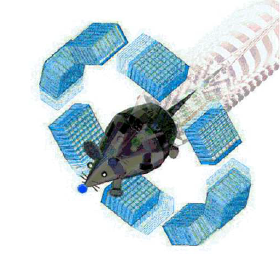
\includegraphics[width=.5\textwidth]{figs/gate_logo.png}
\end{center}

\vspace*{1cm}
\begin{center}
Version 1.0\\
\vspace*{0.5cm}
\today
\end{center}
%\end{tabular*}

\vspace*{5.0cm}
%\begin{center}
%{\normalsize
%Soutenue le 19 Septembre 2014 devant le Jury compos\'{e} de :\\

%\begin{tabular}{lll}
%Mme. & Vera LUTH & Rapporteur\\
%M. & Urs LANGENEGGER & Examinateur\\
%Mme. & Svjetlana FAJFER & Examinateur\\
%M. & Guy WILKINSON & Rapporteur \\
%M. & Achille STOCCHI & Pr\'{e}sident \\
%Mme. & Marie-H\'{e}l\`{e}ne SCHUNE   & Directrice de th\'{e}se \\
%M. & Benoit VIAUD & Examinateur\\
%\end{tabular}
%}
%\end{center}
\vspace{\fill}



\vspace*{1.5cm}
\vspace{\fill}
\endgroup
\end{titlepage}


\pagestyle{empty}  % no page number for the title 

%%%%%%%%%%%%%%%%%%%%%%%%%%%%%%%%
%%%%%  EOD OF TITLE PAGE  %%%%%%
%%%%%%%%%%%%%%%%%%%%%%%%%%%%%%%%

%  empty page follows the title page ----
\newpage
\setcounter{page}{2}


% %%%%%%%%%%%%% ---------

\renewcommand{\thefootnote}{\arabic{footnote}}
\setcounter{footnote}{0}

%%%%%%%%%%%%%%%%%%%%%%%%%%%%%%%%
%%%%% Table of Content %%%%%%
%%%%%%%%%%%%%%%%%%%%%%%%%%%%%%%%
%%%% Uncomment next 2 lines if desired
%\tableofcontents
%\cleardoublepage


%%%%%%%%%%%%%%%%%%%%%%%%%
%%%%% Main text %%%%%%%%%
%%%%%%%%%%%%%%%%%%%%%%%%%

\pagestyle{fancy} % restore page numbers for the main text

%% Uncomment during review phase.
%% Comment before a final submission.
\linenumbers

% You can include short sections directly in the main tex file.
% However, for larger papers it is desirable to split the text into%
% several semiautonomous files, which can be revised independently.
% This is especially useful when developing a document in
% collaboration with several people, since then different parts can be
% edited independently. This type of file organization is shown here.
%\pagenumbering{gobble}
\clearpage
\newpage
%\input{0-resume}\newpage
%\input{0-abstract}\newpage
%\input{0-synthese}\newpage

%\pagenumbering{roman}
\tableofcontents
\clearpage
%\pagenumbering{gobble}
%\pagenumbering{arabic}
%\input{1-Abstract}
\input{0-Introduction}
\input{2-SM}
\input{3-LHCb}
\input{3a-Variables}
\input{7-D2PiMuMu}
\input{4-Trigger}
%%% untag analysis:
\input{8-D2HHMuMu_untag}
%%%%%%
%%%%%% tag analysis:%
\input{8-D2HHMuMu}
\input{5-TestBeam}
\input{9-Conclusion}

%\cleardoublepage\makeatletter\@openrightfalse\makeatother
\appendix
\input{appendix-for-1-2-selection}
\input{appendix-for-1-4-Fitter}
%\input{appendix-for-1-3-hadronicbackground}
\input{appendix-for-1-4-efficiencies}
\input{appendix-for-1-4a-distr}
\input{appendix-for-1-5-systBDT}
\input{appendix-for-1-L0HadMu}
\input{appendix-for-9-Sensitivity}
%\input{appendix}
%
%% Add in the predefined LHCb symbols
\bibliographystyle{LHCb}
\bibliography{../../../../bib/biblio}
\end{document}


